%\documentclass[12pt]{article}
%\usepackage{amstext,amssymb}
%\usepackage{graphicx}
%\usepackage{times}
%\usepackage{psfig,latexsym}
%\usepackage{amstext,amssymb}
%\usepackage{amsmath}
%\begin{document}
%\newtheorem{theorem}{Theorem}
%\newtheorem{lemma}{Lemma}
%\newtheorem{corollary}{Corollary}
%\newtheorem{proposal}{Proposal}
\newcommand{\nchoosek}[2]{\left(\begin{array}{c}#1\\#2\end{array}\right)}
\chapter[Test Chapter]{Test Chapter}
Many communication systems use a substitution-error correcting
code to encode a binary input message $\mathbf{x}$ into a coded
sequence $\mathbf{c}$ = $C(\mathbf{x})$. The modulated version of
this sequence, corrupted by additive noise, arrives at the
receiver as a waveform $r(t)$,
\begin{equation}\label{eq:rt}
r(t)=\sum_{i} c_i h(t-iT) +n(t),
\end{equation}
where $c_i$ is the $i^{\text{th}}$ %$i^{\text{th}}$
bit of $\mathbf{c}$, $h(t)$ is the modulating pulse, and $n(t)$ is
the noise introduced in the channel.

Upon receiving $r(t)$, the receiver samples it at the times
$\left\{kT_s+\tau_k\right\} $. The samples are fed into the
decoder which produces the most likely input message. In
traditional correlation based receivers, for adequate noise
rejection, it is essential that the decoder be provided with
samples taken at approximately optimal time instances. As the
operating requirements under which timing recovery must be
performed become more stringent, such as lower signal to noise
ratio (SNR) and higher data rates, accurate synchronization
becomes critical for the full utilization of the available coding
gains. Several authors have proposed novel schemes which provide
ways of performing improved timing recovery \cite{liu:02},
\cite{kbek:04}.

When the adequate synchronization is missing, as a consequence of
the initial frequency error or of the accumulated phase error,
some symbol may be sampled more than once. Assuming that the exact
sampling instances are not known, a coded sequence $\mathbf{c}$
can give rise to a whole set of received sampled versions of
$r(t)$. When two distinct sequences $\mathbf{c_1}$ and
$\mathbf{c_2}$ result in the same sampled sequence, it is no
longer possible to uniquely determine the coded sequence or its
pre-image $\mathbf{x}$ from the received sequence, which can occur
even in the noise-free environment.

Codes that correct single insertion or a deletion of a bit were
investigated by Levenshtein in \cite{lev:66} and have been further
studied by Ferreira et al., \cite{ferr:97}, Levenshtein
\cite{lev:92}, Sloane \cite{sloane:00}, among others. Even though
these constructions assure that the code is immune to a deletion
or an insertion of a bit, they do not guarantee any other
desirable properties of standard substitution error correcting
codes, such as linearity and a good minimum Hamming distance.
Concatenated codes, with non negligible rate loss, that correct
synchronization errors have been proposed in \cite{cmnv:03} and
\cite{dmackay:01}.

We adopt a coding theoretic point of view in addressing inadequate
synchronization. We propose to focus on the encoding/decoding
components of the communication system and appropriately modify
these for better compensation of the inadequate synchronization.
The advantage of this approach lies in power and latency savings
over complex timing recovery schemes. The challenge lies in
appropriately modifying a code of interest without incurring
significant rate penalty for the benefit of improved
synchronization error correction capability. In our earlier work
\cite{isit06} we proposed a technique based on expurgation of
array-based LDPC codes which ensures immunity to single repetition
error.



In this paper we propose a general encoding method based on
extending an additive error correction code to include immunity to
multiple synchronization errors as follows. Suppose that $C$
denotes the additive error correction code used for transmission.
Let $\mathbf{c}$ denote a codeword in $C$, and let $n$ be the
codeword length. A binary string $\mathbf{p}$ of length $m$ is
prepended to the codeword $\mathbf{c}$ chosen for transmission,
and the resulting string $\mathbf{t}=[\mathbf{p}~ \mathbf{c}]$ is
sent over the channel. We assume that the channel is additive
white gaussian noise (AWGN). In addition, at most $s$ repetitions
are introduced as a consequence of imperfect timing recovery. As a
result, the receiver performs a decoding algorithm on a sequence
of length $n+m+s$, and its goal is to recover the original
sequence $\mathbf{c}$.

In Section \ref{construction} we present a construction of a
collection of strings immune to $s$ repetitions. Having
established several useful ancillary results in Section \ref{aux},
we then describe in Section \ref{enc} how to construct ``target''
string $\mathbf{t}$ used for transmission based on the codeword
$\mathbf{c}$ and the desired repetition-error correction
capability $s$. We show that, by judiciously applying the
construction in Section \ref{aux}, it is possible to achieve $m$
that is only $O(\log n)$. A decoding algorithm appropriate for
channels with $s$ repetitions and substitution errors based on
using LDPC codes is developed in Section \ref{dec}.



\section{Multiple Repetition Error Correcting
Code}\label{construction}

Let us first introduce a transformation in which we express the
number of runs of a string in terms of the weight of a string in
the transformed domain. For a string $\mathbf{c}$ of length $n$,
let the string $\tilde{\mathbf{c}}$ of length $n-1$ be defined as
$\mathbf{c}T_n$, where $T_n$ is a $n \times (n-1)$ matrix
satisfying\vspace{-0.0in}\begin{equation}\label{eq:t}T_{n}(i,j)=\left\{
\begin{array}{lll}
    1, & \text{if }i = j,j+1\\
    0, & \text{else.} \\
\end{array} \right. \end{equation}
If $\mathbf{c}$ has $r$ runs, then $\mathbf{\tilde{c}}$ has weight
$r-1$, and vice versa. Both $\mathbf{c}$ and its complement
$\mathbf{\overline{c}}$ result in the same $\mathbf{\tilde{c}}$.

 For
a prime number $P$, $P > m$, and an $s$-dimensional vector
$\underline{a}$ of residues mod $P$, let $S(\underline{a},m,P)$ be
the set of binary strings of length $m$ satisfying the following
set of congruency constraints:

\begin{equation}\label{eq1}\begin{array}{lll}S(\underline{a},m,P) = \{ & \mathbf{x}=(x_1, x_2, ... x_m) \in \{0,1\}^m
:\\ {} & \sum_{i=1}^{w(\mathbf{x})+1} f_ib_i \equiv a_1 \text{ mod } P,\\
{} & \sum_{i=1}^{w(\mathbf{x})+1} f_i^2b_i
\equiv a_2 \text{ mod } P,\\
{} & \hspace{0.5in}\vdots\\ {} & \sum_{i=1}^{w(\mathbf{x})+1}
f_i^sb_i \equiv a_s \text{ mod } P\},\end{array}\end{equation}

where $w(\mathbf{x})$ denotes the number of ones in $\mathbf{x}$,
$b_i$ is the number of zeros between the $i-1^{\text{st}}$ and
$i^{\text{th}}$ 1 in $\mathbf{x}$ (here $i=1$ run of zeros is
assumed to precede the leftmost 1 and $i=w(\mathbf{x})+1$ run of
zeros is assumed to follow the rightmost 1 in $\mathbf{x}$), $f_i$
is a ``weighting'' associated with $b_i$ such that each $f_i$
belongs to the residue set mod $P$ and $f_i \neq f_j$ for $i \neq
j$.


\begin{lemma}\textit{The set
$S(\underline{a},m,P)$ is s-insertions of zeros
correcting.}\end{lemma}

\textit{Proof}: Consider $\mathbf{x} \in$ $S(\underline{a},m,P)$.
After experiencing $s$ insertions of zeros, it becomes string
$\mathbf{x'}$. We now show that $\mathbf{x}$ is always uniquely
determined from $\mathbf{x'}$.


Let $i_1 \leq i_2 \leq ... \leq i_s$ be the (unknown) indices of
the bins of zeros that have experienced insertions. For each $j$,
$1\leq j \leq s$, compute $a_j'\equiv \sum_{i=1}^{w(\mathbf{x})+1}
f_i^jb_i' \text{ mod } P$, where $b_i'$ is the size of the
$i^{\text{th}}$ bin of zeros of $\mathbf{x'}$. Since we are
dealing with insertions of zeros, the weight of the string is
unchanged, $w(\mathbf{x'})$ = $w(\mathbf{x})$. Let
\begin{equation}\begin{array}{ll}
a_j'& \equiv \sum_{i=1}^{w+1} f_i^jb_i' \text{ mod } P\\
{}  & \equiv a_j + (f_{i_1}^j+f_{i_2}^j+...+f_{i_s}^j) \text{ mod
}P,
\end{array}
\end{equation}
where $a_j$ is the $j^{\text{th}}$ entry in the residue vector
$\underline{a}$.

By collecting the resulting expressions over all $j$, and setting
$R_j \equiv a_j'-a_j$ mod $P$, we arrive at
\begin{equation}
E_s=\left\{
\begin{array}{ll}
R_1 \equiv f_{i_1}+f_{i_2}+...+f_{i_s} \text{ mod }P\\
R_2 \equiv f_{i_1}^2+f_{i_2}^2+...+f_{i_s}^2 \text{ mod } P\\
\hspace{0.5in}\vdots\\
R_s \equiv f_{i_1}^s+f_{i_2}^s+...+f_{i_s}^s \text{ mod } P.\\
\end{array} \right.
\end{equation}
The terms on the right hand side of the congruency constraints are
known as power sums in $s$ variables. %Let $S_k$ denote the
%$k^{\text{th}}$ power sum mod $p_l$ of $\{i_1,i_2,...,i_t\}$,
%\begin{equation}
%S_k\equiv i_1^k+i_2^k+...+i_t^k \text{ mod }p_l,
%\end{equation}
%and
Let $\Lambda_k$ denote the $k^{\text{th}}$ elementary symmetric
function of  $\{f_{i_1},f_{i_2},...,f_{i_s}\}$ mod $P$,
\begin{equation}
\Lambda_k \equiv \sum_{v_1<v_2<...<v_k} f_{v_1}f_{v_2}\cdots
f_{v_k} \text{ mod } P.
\end{equation}
Using Newton's identities over $GF(P)$ which relate power sums to
symmetric functions of the same variable set, and are of the type
\begin{equation}\label{newton}
R_k-\Lambda_{1}R_{k-1}+\Lambda_{2}R_{k-2}-...+(-1)^{k-1}\Lambda_{k-1}R_{1}+(-1)^kk\Lambda_{k}
=0,
\end{equation}
for $k \leq s$, we can obtain an equivalent system of $s$
equations:
\begin{equation} \label{eq:dcoeff}
\widetilde{E}_s=\left\{
\begin{array}{ll}
d_1 \equiv \sum_{j=1}^s f_{i_j} \text{ mod }P\\
d_2 \equiv \sum_{j<k} f_{i_j} f_{i_k}\text{ mod }P\\
\hspace{0.5in}\vdots \\
d_s \equiv \prod_{j=1}^s f_{i_j} \text{ mod }P,
\end{array} \right.
\end{equation}
where each residue $d_k$ is computed recursively from
$\{d_1,...,d_{k-1}\}$ and $\{R_1,R_2,...,R_k\}$. This may be done
because, in each $k^{\text{th}}$ equation of the $s$ equations of
type (\ref{newton}) we use, the coefficient of $\Lambda_k$ is
nonzero.

Consider the expression:\vspace{-0.1in}
\begin{equation}\label{eq:p0} \prod_{j=1}^s(x-f_{i_j})\equiv 0 \text{ mod } P,
\end{equation}
and expand it into the form
\vspace{-0.1in}\begin{equation}\label{eq:p}
x^t+c_{t-1}x^{t-1}+...+c_1x+c_0 \equiv 0 \text{ mod } P.
\end{equation}
Since (\ref{eq:p0}) equals (\ref{eq:p}), by comparison with
(\ref{eq:dcoeff}) we see that $d_k \equiv (-1)^kc_{t-k} \text{ mod
} P$. We may then solve for the roots of (\ref{eq:p}) to get the
desired set of indices of weightings
$\{f_{i_1},f_{i_2},...,f_{i_s}\}$. Since different $f_{i_j}$'s
correspond to different bin indices, we may also recover the set
$\{{i_1},{i_2},...,{i_s}\}$, and from it the string $\mathbf{x}$
by deleting zeros from the bins of zeros indexed by the set
$\{{i_1},{i_2},...,{i_s}\}$. Hence $\mathbf{x}$ is always uniquely
recovered from $\mathbf{x'}$.$\hfill\blacksquare$

%
%As already mentioned, the weight of the transmitted string does not
%change during the transmission. Thus if one is interested in
%maximizing the size of the collection of strings capable of
%overcoming $s$ insertions of zeros using the above construction, one
%may partition the set $\{0,1\}^m$ by the weight. Then one can select
%the smallest prime $P_l$, $P_l>l$ in (\ref{eq1}) for each weight $l$
%(as opposed to a single $P$ for all weight groups).

Therefore, the pre-image of $S(\underline{a},n-1,P)$ under $T_n$
gives an $s$ repetitions correcting set.


\section{Auxiliary results}\label{aux}
We now prove some auxiliary results which will be used in the
following section on encoding.

\begin{lemma}\label{generates} For an integer $P$, each residue $r$ mod $P$ can be expressed as a
sum of a subset of elements of the set
$A_{z,P}=\{[z]_P,[2z]_P,[2^2z]_P,...,[2^{G}z]_P\}$ where
$G=\lfloor \log_2 P \rfloor $, $z$ is an arbitrary non zero
residue mod $P$ and the notation $[x]_P$ indicates the residue mod
$P$ congruent to $x$ .
\end{lemma}

\noindent \textit{Proof:} Observe that
$A_{1,P}=\{1,2,2^2,...,2^{G}\}$. We first show that each residue
$r$ mod $P$ can be expressed as a sum of a subset of elements of
the set $A_{1,P}$. Note that each residue $i$, $0 \leq i \leq
2^G-1$ (mod $P$) can be expressed as a sum of a subset, call it
$Q_i$, of the set $\{1,2,2^2,...,2^{G-1}\}$. Adding $2^G$ to the
sum of each $Q_i$, for $1 \leq i \leq 2^G-1$, generates the
residues $\{2^G, 2^G+1,...,P-1 \}\cup \{1,2,...2^G-1\}$. As a
result every residue mod $P$ can be expressed as a sum of a subset
of $A_{1,P}=\{1,2,2^2,...,2^{G}\}$.

Suppose there exists an element $r$ which cannot be expressed as a
sum of a subset of elements of $A_{z,P}$, for $z>1$, that is $r
\neq \sum_{i=0}^G \epsilon_i z 2^i \mod P$, for all choices of
$\{\epsilon_0,...,\epsilon_G\}$, $\epsilon_i \in \{0,1\}$. Then
the residue $r' = rz^{-1} \neq \sum_{i=0}^G \epsilon_i 2^i \mod
P$, for all choices of $\{\epsilon_0,...,\epsilon_G\}$,
$\epsilon_i \in \{0,1\}$, which contradicts the result from the
previous paragraph.\hfill$\blacksquare$

Suppose $P$ is a prime number such that $i|P-1$. Suppose the
equation $x^i\equiv a \mod P$ has a solution, $1 \leq a \leq P-1$.
Then the equation $x^i\equiv a \mod P$ has $i$ distinct solutions
\cite{apostol} and we may call them $x_1$ through $x_i$.
\begin{lemma}\label{sums}
The sum $\sum_{k=1}^i x_k^j \equiv 0 \mod P$ for $1 \leq j \leq
i-1$.
\end{lemma}
\noindent \textit{Proof:} Let us consider the equation $x^i \equiv
a \mod P$. Using Vieta's formulas over $GF(P)$ it follows that
$\Lambda_{j}=0$ for $0 \leq j \leq i-1$. Using Newton identities
over $GF(P)$ it then follows that
 $\sum_{k=1}^i x_k^j \equiv 0 \mod P$ for $1 \leq j \leq
i-1$.\hfill$\blacksquare$

For a prime number $P$ for which $i|P-1$, and $i<P-1$, let
$Q_i(P)$ be the set of distinct $i$th power residues mod $P$, let
$N_i(P)$ be the set of distinct $i$th power non residues mod $P$.
We also state the following convenient result.
\begin{lemma}\label{main}
Each $n \in N_i(P)$ can be expressed as a sum of two distinct
elements of $Q_i(P)$ in at least $P/(2k^2)-\sqrt{P}/2-3$ ways.
\end{lemma}
\noindent \textit{Proof:} The result follows from \cite{huavan:49}
which states that over $GF(P)$ the equation
\begin{equation}\label{hua} x^k+y^k=a
\end{equation} where $x,y,a \in GF(P)$ and nonzero and $0 < k <P-1 $
has at least $P-(k-1)^2\sqrt{P}-2(k-1)^2$ solutions. Noting that
$k$ distinct values of $x$ result in the same $x^k$, accounting
for the symmetry of $x$ and $y$, and omitting the case $x^k=y^k$
we obtain the lower bound on the number of solutions as
$P/(2k^2)-\sqrt{P}/2-3$. \hfill$\blacksquare$

Equations of the type in (\ref{hua}) were also studied by Weil
\cite{weil:49}.
\section{Encoding}\label{enc}

Let $s$ denote the target synchronization error correction
capability. The goal of this section it to provide an explicit
encoding scheme which based on the coded message $\mathbf{c}$
produces a fixed length prefix $\mathbf{p}$, where $\mathbf{p}$ is
a function of $\mathbf{c}$, such that the string $\mathbf{t}=[
\mathbf{p} ~ \mathbf{c} ]$ satisfies first $s$ congruency
constraints previously described (used for the recovery from
synchronization errors) in section~\ref{construction}. Using
judiciously chosen prefix, we will show that this will be possible
for $m=|\mathbf{p}|=O(\log n)$. As a result the transmitted string
will have asymptotically negligible rate loss compared to the
starting code $C$ while providing improved immunity to
synchronization errors.

 Let $w$ be
the design parameter, $w \in \mathbb{N}$, which determines the
sizes of the bins in the the substring $\mathbf{p}$ of
$\mathbf{t}$ under $T_{m+n}$ transformation. This parameter will
be exploited in the decoding of the $\mathbf{p}$ string, as
explained in Section~\ref{dec}.

 Let $P$ be a prime number chosen such that $P$ is
$c_1n < P< c_2n$, for appropriately chosen constants $c_1$ and
$c_2$.  We choose $c_1$ such that $c_1n>n+s(s+1)(\lfloor\log
P\rfloor+1)$ and $c_2$ sufficiently large such that
$lcm(2,3,\dots,s)|P-1$.


 We
construct $\mathbf{p}$ of length $m$ such that in
$\mathbf{\tilde{t}}=[\mathbf{p}~ \mathbf{c}]T_{m+n}$ the leftmost
substring $\mathbf{\tilde{t}}(1,m)$ (here and in the remainder
$\mathbf{x}(p,q)$) denotes a substring of $\mathbf{x}$ spanning
positions $p$ and $q$) has weight \begin{equation}\label{sum1}
1+\sum_{i=1}^s i\left[ 2(G+1)-\lceil(G+1)/i \rceil
\right]\end{equation} and ends in `1'. Since the pre-image under
$T_m$ contains two strings (which are complements of each other)
we let $\mathbf{p}$ be the one for which
$\mathbf{p}(n)=\overline{\mathbf{c}(1)}$ (here and in the
remainder $\mathbf{x}(q)$ denotes the bit in the $q^{\text{th}}$
position in $\mathbf{x}$, and $\overline{\mathbf{x}(q)}$ denotes
the complement of the bit $\mathbf{x}(q)$). %As a result the
%$(G+2)^{\text{st}}$ bin in $\mathbf{t}$ is fully contained in the
%substring $\mathbf{p}$, and the $(G+3)^{\text{nd}}$ run in
%$\mathbf{t}$ is fully contained in the substring $\mathbf{c}$.
Let $b_i$ is the number of zeros between the $(i-1)^{\text{st}}$
and $i^{\text{th}}$ 1 in $\mathbf{\tilde{t}}$. This run of zeros
will be referred to as the $i^{\text{th}}$ bin. Let $M$ be the
total number of bins in $\mathbf{\tilde{t}}$.


%Since $\mathbf{p}(n)=\overline{\mathbf{c}(1)}$, the
%${G+2}^{\text{nd}}$ bin is fully contained in the
%$\mathbf{\tilde{p}}$ portion of $\mathbf{\tilde{t}}$, and likewise
%the ${G+3}^{\text{nd}}$ bin is fully contained in the
%$\mathbf{\tilde{c}}$ portion of $\mathbf{\tilde{t}}$.





Let $R(P)$ denote the reduced set of residues mod $P$. For each
$i, 1 \leq i \leq s$, since $i | P-1$ by construction, $Q_i(P)$ is
of size $(p-1)/i$ \cite{apostol}. Consider the set
$A_{z_i,P}=\{[z_i]_P,[2z_i]_P,[2^2z_i]_P,...,[2^{G}z_i]_P\}$ where
$G=\lfloor \log_2 P \rfloor $ and $z_i \in Q_i(P)$. By Lemma
\ref{generates} each residue in $R(P)$ can be written as a linear
combination of some elements in $A_{z_i,P}$.

Moreover, each element in $A_{z_i,P}$ either belongs to $Q_i(P)$
or, if not, can be expressed as a sum of two distinct elements of
$Q_i(P)$ in at least $P/(2i^2)-\sqrt{P}/2-3$ ways by Lemma
\ref{main}. Replace each $i$th power non residue $x$ in
$A_{z_i,P}$ by two $i$th power residues, the sum of which is $x$,
and such that no  $i$th power residue participates in the sum of
more than  one such element, and such that itself is not an
original element of $A_{z_i,P}$. Let $Y_i(z_i)$ be the resulting
set. It is of size $2(G+1)-\lceil (G+1)/i \rceil$. We have thus
obtained the set $Y_i(z_i)$ of size $O(\log P)$ and such that all
elements in $R(P)$ can be expressed as a linear combination of
elements of $Y_i(z_i)$, by Lemma \ref{generates}.

Let $V_i(z_i)$ for $1 \leq i \leq s$ be such that each $V_i(z_i)$
is of size $i \times Y_i(z_i)$ and contains all $ith$ roots of
elements of $Y_i(z_i)$. Select $z_1$ through $z_s$ such that
$V_i(z_i) \cap V_j(z_j) = \emptyset$ for $i \neq j, 1 \leq i,j
\leq s $, which is possible for $P$ large enough. Along with the
zero weighting, the elements of $V_i(z_i)$ for $1 \leq i \leq s$
are reserved to be weightings of the first
$|V_1(z_1)|+\dots+|V_s(z_s)|+1$ bins in $\mathbf{t}$ which are
made to entirely and only arise from runs in $\mathbf{p}$. Note
that for $\mathbf{\tilde{p}}$ the number of bins equals the
weight, which is (\ref{sum1}), as required. For notational
simplicity let $L=|V_1(z_1)|+\dots+|V_s(z_s)|+2$.



 Let
\begin{eqnarray}\label{code1} {a'}_1 &\equiv& \sum_{i=L}^M b_i f_i
\text{ mod } P, \\ {a'}_2 &\equiv& \sum_{i=L}^M b_i f_i^2 \text{
mod } P\\ &\vdots& \\
\label{codes}{a'}_s &\equiv& \sum_{i=L}^M b_i f_i^s \text{ mod }
P\end{eqnarray}

where $f_i$ in (\ref{code1}) through (\ref{codes}) are chosen in
the increasing order from the set $R(P)\setminus \{V_1(z_1) \cup
\dots \cup V_s(z_s) \}$, which is possible by the lower bound on
$P$. Note that $M-L+1 \leq n $. We may think of ${a'}_1$ through
${a'}_s$ as the contribution of the codeword to the overall
congruency value. We now show that it is always possible to
achieve
\begin{eqnarray}\label{s1} a_1 &\equiv& \sum_{i=1}^M b_i f_i
\text{ mod } P, \\ a_2 &\equiv& \sum_{i=1}^M b_i f_i^2 \text{
mod } P\\ &\vdots& \\
a_s &\equiv& \sum_{i=1}^M b_i f_i^s \text{ mod }
P\label{s2}\end{eqnarray}

for arbitrary but fixed values $a_1$ through $a_s$ irrespective of
the values ${a'}_1$ through ${a'}_s$, where $b_i$ is either $0$ or
$w$ for $1 \leq i \leq L-1$, and where $f_L=0$.

The encoding is recursive and proceeds as follows.

Let $l$ be the $l$th level of recursion for $l=1$ to $l=s$. The
$l$th level ensures that the $l$th congruency constraint is
satisfied without altering previous $l-1$ levels.
 At each level $l$, starting with $l=1$ and while $l \leq s$:
\begin{enumerate}
 \item Select a subset $F_{l}$ of $V_l(z_l)$ such that $\sum_{k \in F_l} k^lw \equiv a_l - {a'}_l -
\sum_{i=1}^{l-1} d_{i,l} \mod P$. (For $l=1$, $\sum_{k \in F_1} kw
\equiv a_1 - {a'}_1 \mod P$.)\item Let $d_{l,j} \equiv \sum_{k \in
F_l} k^jw \mod P$ for $l+1 \leq j\leq s$. \item For each $i$, $1
\leq i \leq |V_l(z_l)|$, for which $f_i \in F_l$ we set $b_i=w$,
and for each $i$, $1 \leq i \leq |V_l(z_l)|$, for which $f_i
\notin F_l$ we set $b_i=0$, where $w$ is a fixed integer $w \geq
1$. \item Proceed to level $l+1$.
\end{enumerate}

After the level $s$ is completed, let $b_L=w(\sum_{i=1}^s
|V_i(z_i)|- |F_{i}|)$. The purpose of this bin with weighting zero
is to ensure that the overall string $\mathbf{t}$ has the same
length irrespective of the structure of the starting codeword
$\mathbf{c}$.

The existence of $F_l, F_l \subseteq V_l(z_l)$ in Step 1) follows
from Lemma~\ref{generates} and Lemma~\ref{main}. Observe that by
Lemma~\ref{sums} the contribution to each congruency sum for
levels $1$ through $l-1$ of the elements of $F_l$ is zero. Hence,
once the target congruency value is reached for a particular
level, it will not be altered by establishing congruencies at
subsequent levels.
\section{Decoding}\label{dec}

Assume that based on a codeword $\mathbf{c}$ a string
$\mathbf{t}=[\mathbf{p} ~ \mathbf{c}]$ is constructed using the
encoding procedure outlined above, such that $\mathbf{t}$
satisfies (\ref{s1}) through (\ref{s2}). Assume that $\mathbf{t}$
is transmitted over an AWGN channel, which in addition introduces
$s$ repetitions. The received sequence $\mathbf{r}$ is of length
$|\mathbf{t}|+s$ bits.

The decoding consists of the following steps:
\begin{enumerate}
\item Decode $\mathbf{p}$ portion of $\mathbf{r}$. \item Determine
the contribution of  $\mathbf{p}$ to (\ref{s1}) through
(\ref{s2}). \item Decode $\mathbf{c}$ portion of $\mathbf{r}$.
\item Determine the contribution of  $\mathbf{c}$ to (\ref{s1})
through (\ref{s2}) and if consistent with the target values $a_1$
through $a_s$, declare successful decoding.
\end{enumerate}

In particular:

Step (1). By construction, all but one run in $\mathbf{p}$ is
either of length $1$ or $w+1$. Upon receiving corrupted version of
$\mathbf{p}$ we may perform brute force search to find the most
likely $\mathbf{\hat{p}}$ since its length is only logarithmic in
the codeword length by construction.

Step (2). Compute $\hat{a}^{''}_k \equiv \sum_{i=1}^{L-1}
\hat{b}_i \hat{f}_i^k \mod P$ for $1\leq k \leq s$, where
$\hat{b}_i$ and $\hat{f}_i$ are obtained from $\mathbf{\hat{p}}$.

Step (3). We introduce auxiliary variables $G$, an $s$-dimensional
vector $(g_1,\dots,g_s)$ which takes values $\in \{1,...,n\}^s$,
and $L_i$, for $\forall$ $i \in [1,n]$, such that $L_i \in
\{-s,-s+1,...,-1,0,1,...,s-1,s\}$. The variable $G$ denotes the
positions of the repetitions, and $L_i$ denotes the relative
location of the $i^{\text{th}}$ bit with respect to the
repetitions. Let $\mathbf{y}_1^{n+s}=\mathbf{r}_{m+1}^{m+n+s}$.

Write \begin{equation}\label{marg}P(x_i| \mathbf{y}_1^{n+s}) =\\
\sum_G \sum_{L_1^n} \sum_{x_1^n \backslash x_i} P(x_1^n,L_1^n,G
|\mathbf{y}_1^{n+s}).\end{equation}

Group the variables as shown in Fig. 1., for $1 \leq i \leq n$ and
$1 \leq k \leq M_c$, where $M_c$ is the total number of checks.
Note that $\mathbf{y}_1^{n+s}$ is viewed as evidence.
\begin{figure}\label{ta1}
\hspace{-0.0in}\small\begin{tabular}{|c|c|}
  \hline
  % after \\: \hline or \cline{col1-col2} \cline{col3-col4} ...
   \text{local domain} & \text{local function} $\varphi(\cdot)$\\
  \hline
   $\{G\}$ & 1 \\\hline
   $\{G,L_i\}$ & $1\left[L_i=s\cdot 1(g_1<...<g_s\leq i-1)+\right.$\\
   {} & $\left. +\dots +L_i=-s\cdot 1(g_s>...>g_1\geq i+1)\right]$\\
   \hline
   $\{L_i,x_i\}$ &
   $P(y_i|x_i)1(L_i=-s)$+\\{} & $P(y_i|x_i)P(y_{i+1}|x_i)1(L_i=-s+1)+...+$\\
   {} & $P(y_{i+s-1}|x_i)P(y_{i+s}|x_i)1(L_i=s-1)$\\{}&+$P(y_{i+s}|x_i)1(L_i=s)$\\\hline
   $\{x_i\}$ & 1\\\hline
   $\{c_k,(x_j,j \in \mathcal{N}_k)\}$ & $1(c_k =\oplus_{j \in
   \mathcal{N}_k} x_j)$\\
  \hline
\end{tabular}\caption{Local domains and functions for Step 3.}
\end{figure}

The junction graph corresponding to these local domains is shown
in Fig. 2, and has the bidirectional edges between:\begin{itemize}
\item $\{G \}$ and $\{G, L_i\}$ for each $1 \le i \le n$, \item
$\{G, L_i\}$ and $\{ L_i, x_i\}$ for each $1 \le i \le n$,  \item
$\{ L_i, x_i\}$ and $\{c_k, (x_i, i \in {N}_k )\}$, for each pair
$(i,k)$ such that $i \in {N}_k$, and \item $\{x_i\}$ and
$\{L_i,x_i\}$ for each $1 \le i \le
n$.\end{itemize} %Then,

%\begin{equation}\hspace{0.4in}\label{joint}\begin{array}{ll}
%\sum_G \sum_{L_1^n} \sum_{x_1^n \backslash x_i}
%P(x_1^n,L_1^n,G,y_1^{n+1}) \approx
%\\\hspace{-0.4in} \sum_{L_i} \varphi(L_i,x_i)\sum_G\varphi(G,L_i)\prod_{j=1,j
%\neq i}^n  \sum_{L_j} \varphi (G,L_j) \\ \times \sum_{x_j}
%\varphi(L_j,x_j) \prod_{k \in \mathcal{N}_i} 1(c_k =\oplus_{j \in
%   \mathcal{N}_k} x_j)\vspace{-0.1in}\end{array}\end{equation}
%where $\varphi(\cdot)$ denotes the local function of the appropriate
%variables listed in Fig.1 and the approximation comes from ignoring
%the cycles in the graph.

\begin{figure}
%\vspace{0.0in}\hspace{0.0in}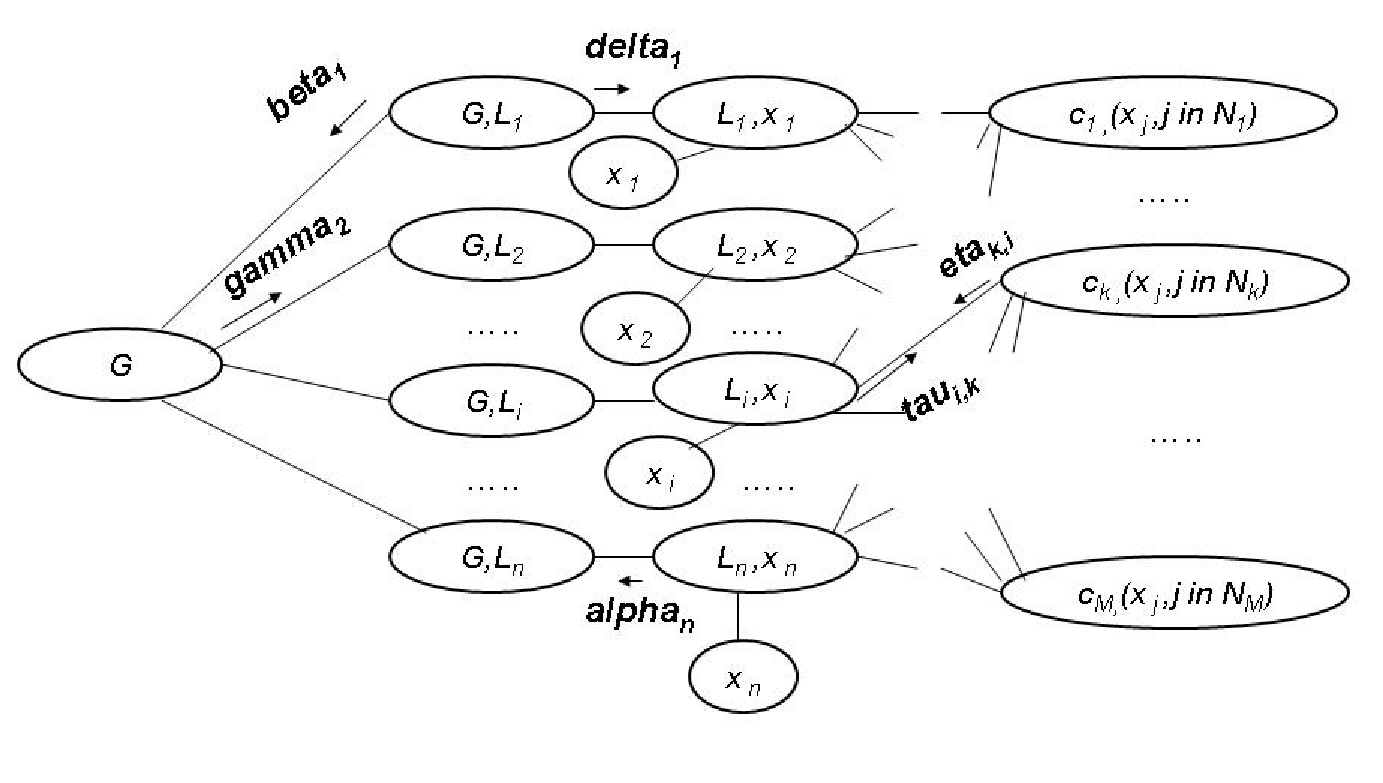
\includegraphics[width=3.0in,height=1.9in]{fig7.eps}
\caption{Junction graph for Step 3.}
\end{figure}

Observe that
\begin{equation}\begin{array}{lll}
P(x_1^n,L_1^n,G|\mathbf{y}_1^{n+s}) \propto \\\varphi(G) \prod_{i}
\varphi(G,L_i) \prod_{i} \varphi(L_i,x_i) \prod_i\varphi(x_i)
\prod_k \varphi(c_k,(x_j, j \in \mathcal{N}_k)).\end{array}
\end{equation}

We may use a message passing algorithm as in \cite{aji} to try to
evaluate  $P(x_i|\mathbf{y}_1^{n+s})$.

Let all messages be initialized to 1, and let $\alpha_j(L_j)$ be
the message sent from $\{L_j,x_j\}$ to $\{G,L_j\}$ at some stage.

The message $\beta_j(G)$ from $\{G,L_j\}$ to $\{G\}$ is then
$\beta_j(G)=\sum_{L_j}\varphi (G,L_j)\alpha_j(L_j)$, and the
message $\gamma_i(G)$ sent from $\{G\}$ to $\{G,L_i\}$ is
$\prod_{j \in \{1,n\}\backslash i} \beta_j(G)$. Finally, the
message from $\{G,L_i\}$ to $\{L_i,x_i\}$ is
$\delta_i(L_i)=\sum_G\varphi(G,L_i)\gamma_i(G)$.

The message $\tau_{j,k}(x_j)$ sent from $\{L_j,x_j\}$ to $\{c_k
(x_j, j \in \mathcal{N}_k)\}$ is $\sum_{L_j}\varphi(L_j,x_j)
\delta_j(L_j)\prod_{l \in \mathcal{N}_j \backslash k}
\eta_{l,j}(x_j)$, where $\eta_{l,j}(x_j)$ is the message from
$\{c_l,(x_j, j\in \mathcal{N}_l)\}$ to $\{L_j,x_j\}$ and is
$\sum_{x_i,i\in \mathcal{N}_l\backslash j}\varphi(c_l, (x_i, i \in
\mathcal{N}_l)) \prod \tau_{i,l}(x_i).$

The message $\alpha_j(L_j)$ is updated to $\sum_{x_j}
\varphi(L_j,x_j) \prod_{k \in \mathcal{N}_j}\eta_{k,j}(x_j)$, and
message exchange continues as above.

As a result, from (\ref{marg}) one gets \begin{equation}P(x_i|
\mathbf{y}_1^{n+s}) \approx
\sum_{L_i}\varphi(L_i,x_i)\delta_i(L_i)\prod_{k \in \mathcal{N}_i}
\eta_k (x_i),\end{equation} and we also have
\begin{equation}
P(G=\underline{g}|\mathbf{y}_1^{n+s}) \approx \prod_{i=1}^n
\beta_i(\underline{g}).
\end{equation}
Even though there are $O(n)$ computations each involving $O(n)$
variables per global iteration step, computational complexity can
be reduced from $O(n^2)$ to $O(n)$ with appropriate organization
of calculations. In particular, $\delta$'s can be computed
directly from $\alpha$'s. For details please see \cite{tech:07}.


The messages $\tau_{j,k}$ and $\eta_{k,j}$ are analogous to
messages computed in a traditional message passing algorithm on a
bipartite graph, so their complexity is also $O(n)$.

Step (4). Compute $\hat{a}'_k \equiv \sum_{i=L}^{M} \hat{b}_i
\hat{f}_i^k \mod P$ for $1\leq k \leq s$, where $\hat{b}_i$ and
$\hat{f}_i$ are obtained from $\mathbf{\hat{c}}$. If
$\hat{a}'_k+\hat{a}^{''}_k \equiv a_k \mod P$ for $1\leq k \leq s$
declare successful decoding.
\subsection{Simulation results}
To be filled in-in progress.\vspace{0in}
\section{Concluding remarks}
We proposed a technique for modifying additive error correction
codes when varying sampling rate causes repetition of symbols. We
presented an encoding scheme which relies on introducing a
carefully chosen prefix such that the overall string (consisting
od the prefix and the codeword) is immune to repetition errors.
The prefix length is only logarithmic in the codeword length. We
also gave a companion message passing algorithm suitable for
decoding of LDPC codes under multiple repetitions and with such a
prefix.

\section*{Acknowledgment}
% optional entry into table of contents (if used)
%\addcontentsline{toc}{section}{Acknowledgment}
The authors would like to thank Marvell Semiconductor Inc. and
U.C. MICRO program for supporting their research.

\begin{thebibliography}{10}
\bibitem{aji}
S. Aji and R. McEliece, ``The generalized distributive law",
\emph{IEEE Trans.  Inform. Theory} vol.\ 46(2), pp.~325--43, March
2000.
\bibitem{apostol} T. M. Apostol, ``\emph{Introduction to Analytic Number
Theory}'', Springer-Verlag, NY, 1976.
\bibitem{cmnv:03}
G. Chen, M. Mitzenmacher, C. Ng and N. Varnica,``Concatenated
codes for deletion channels,'' In \emph{Proc. of the IEEE
International Symposium on Information Theory} 2003, Yokohama,
Japan, p.~218.
\bibitem{dmackay:01}
M.C. Davey and D.J.C. MacKay, ``Reliable communication over
channels with insertions, deletions and substitutions,''
\emph{IEEE Trans. on Information Theory} vol.\ 47(2), pp.~687-698,
Feb. 2001.
\bibitem{isit06} L. Dolecek and V. Anantharam, ''A synchonization
technique for array-based LDPC codes'', \emph{Int. Symp. on
Information Theory}, Seattle, WA, 2006.
\bibitem{tech:07} L. Dolecek and V. Anantharam, ``On reliable communication over channels
with varying sampling rate,'' available at
www.eecs.berkeley.edu/\~{}dolecek/papers
\bibitem{ferr:97}
H.C. Ferreira, W.A. Clarke, A.S.J. Helberg, K.A.S. Abdel-Ghaffar
and A.J. Han Vinck, ``Insertion/deletion correction with spectral
nulls,'' \emph{IEEE Trans. on Information Theory} vol.\ 43(2),
pp.~722--732, March 1997.
\bibitem{huavan:49}
L. K. Hua and H. S. Vandiver, ``Characters over certain types of
rings with applications to the theory of equations in a finite
field'', \emph{Proc. Nat. Acad. Sci. USA}, vol. 35, pp.~481-487,
1949.
\bibitem{lev:66}
V. I. Levenshtein,``Binary codes capable of correcting deletions,
insertions and reversals,'' \emph{Sov. Phys.-Dokl.}, vol.\ 10(8),
pp.~707--710, Feb. 1966.
\bibitem{lev:92}
V. I. Levenshtein, ``On perfect codes in deletion and insertion
metric,'' \emph{Discrete Math. Appl.}, vol.\ 2(3), pp.~241--258,
1992.
\bibitem{liu:02}
J. Liu, H. Song and B.V.K.V. Kumar, ``Symbol timing recovery for
low-SNR partial response recording channels," In \emph{Proc.
GLOBECOM 2003}, Nov. 2002, pp. 1141 -- 1145, San Francisco, CA,
USA.
\bibitem{kbek:04}
P. Kovintavewat, J. R. Barry, M. F. Erden and E. Kurtas,
``Per-survivor timing recovery for uncoded partial response
channels,''\emph{Proceedings of the IEEE International Conference
on Communications} 2004, Paris, France.
\bibitem{sloane:00}
N.J.A. Sloane, ``On single deletion correcting codes,'' 2000.
Available at http://www.research.att.com/\~{ }njas/doc/dijen.pdf
\bibitem{weil:49}
A. Weil, ''Numbers of solutions of equations in finite fields", in
\emph{Bull. Amer. Math. Soc}, vol. 50, pp.~497--508, 1949.
\end{thebibliography}
%\end{document}
